\documentclass{article}

\usepackage{graphicx}
\usepackage{caption}
\usepackage{subcaption}
\usepackage{booktabs}
\usepackage{csvsimple}

\usepackage{tikz}
\usetikzlibrary{bayesnet}
\usetikzlibrary{positioning}

\title{Predicting positions using Independence Graphs}
\author{Volker Strobel}
\date{\today}

\graphicspath{{img/}}

\begin{document}
\maketitle

% Inducing Features of Random Fields (Pietra)

% I can start with one feature and
% successively include more and more features, until my prediction
% becomes better and better.

% Test on hold-out test see

% Archimedean copulas are an associative class of copulas. Most common
% Archimedean copulas admit an explicit formula, something not
% possible for instance for the Gaussian copula. In practice,
% Archimedean copulas are popular because they allow modeling
% dependence in arbitrarily high dimensions with only one parameter,
% governing the strength of dependence

% Linear regression

% Greedy approach for feature inclusion

% MSE minimizes the expected error
% Another error function minimizes the model

% http://www.r-bloggers.com/modelling-dependence-with-copulas-in-r/

\begin{abstract}
  In this report, we use variants of linear regression, independence
  graphs, and vine copulas, to analyze the distribution and predictive
  power of image features--color and edge histograms. We compare the
  predictive power of the used models using the mean absolute error of
  the predictions on a hold out test set. We study the associated
  uncertainty in the predictions and give indications, how the
  proposed model can be used in the physical world.
\end{abstract}

\section{Introduction \& Problem Statement}

% This could be used in the context of a UAV flight...

The goal of computer vision is to make machines see---for example, for
the purpose of object detection, image restoration, or
\emph{localization}. In this report, we consider the following
problem:

Based on a given patch of an image, we would like to predict, where
the patch was taken in a larger image---the map image. While existing
approaches extract key features of the current patch and the map
image, these approaches are usually computationally complex and do not
allow for in-depth analysis for the problem. 

image patches from a given map image are generated. These images
simulate camera images that could be obtained during a flight with a
UAV. Therefore, we like to address the problem based on two
approaches: (i) modify the environment (i.e., the map image) to make it
better suited for the used approach, and (ii) modify the approach to
make it better suited to the given map image. 

The goal is to learn a model and predict the location of unseen image
patches. Figure~\ref{fig:generation} shows the process of data set
generation.

\begin{figure}
  \centering
  \begin{subfigure}[b]{0.4\textwidth}
    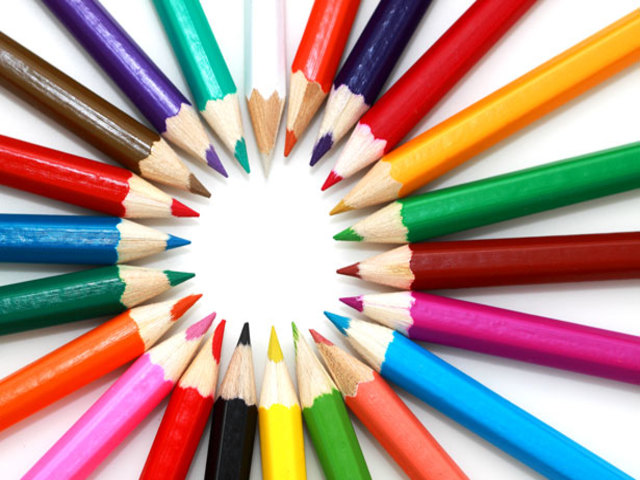
\includegraphics[width=\textwidth]{pencils}
    \captionof{figure}{Map image}
    \label{fig:mapimage}
  \end{subfigure}%
~
  \begin{subfigure}[b]{0.4\textwidth}
    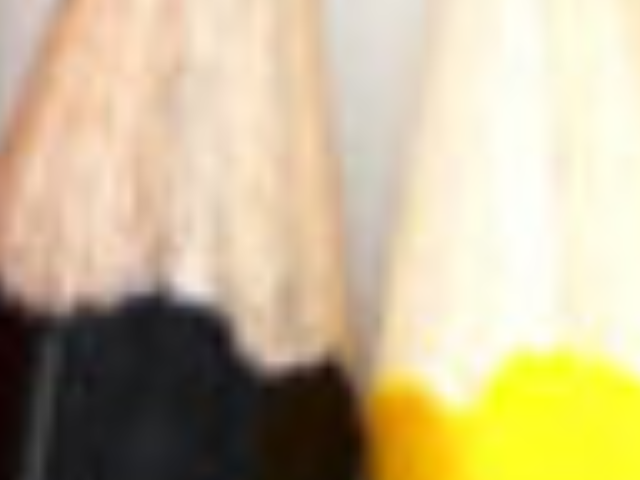
\includegraphics[width=\textwidth]{patches}
    \captionof{figure}{Random image patch}
    \label{fig:patch}
  \end{subfigure}
  \caption{Figure~\ref{fig:mapimage} Shows the map image that is used
    for generating the image patches. Figure~\ref{fig:patch} shows one
    sample of the $N = 1000$ image patches that were generated for the
  generation of the data set.}
\label{fig:generation}
\end{figure}

By construction, we know that $x$, $y$ are independent, since the
positions were sampled from independent uniform distributions.

This leads to the data set that can be found in the appendix.

% The presented approach uses simulated data but should be able to
% generalize to real world models.  In a first step, we will select
% suitable features in an iterative approach.


In this setting, the availability of the data is not a problem and new
data can be easily generated. What we would like to have is a
dependency model that is able to capture the multivariate distribution
of the sample data. This approach is based on Sklar's theorem that
states that multivariate distribution can be described by marginal
distributions and the dependence structure----the copulas. Using
bivariate copulas as building blocks, more complex interaction
structures can be achieved by building \emph{vine copulas}--nested
sets of connected trees.

\section{Methods}

In our first model, we use three features: the average red, green, and
blue color per image patch. The data set based on $N = 1000$ image
patches can be found in the appendix.

\begin{table}[h]
  \centering
  \begin{tabular}{l|rrrrr}
    red   & 3558  &       &      &       &       \\
    green & 1578  & 3354  &      &       &       \\
    blue  & 1219  & 2749  & 4016 &       &       \\
    x     & -1199 & -427  & -343 & 22900 &       \\
    y     & -871  & -389  & 616  & 467   & 12204 \\
    \midrule
    means & 180   & 154   & 145  & 244   & 192   \\
    \midrule
          & red   & green & blue & x     & y
  \end{tabular}
  \caption{The sample variance matrix of the data set}
\end{table}

\begin{table}[h]
  \centering
  \begin{tabular}{l|rrrrr}
    red   & 1.00  &       &       &      &      \\
    green & 0.46  & 1.00  &       &      &      \\
    blue  & 0.32  & 0.75  & 1.00  &      &      \\
    x     & -0.13 & -0.05 & -0.04 & 1.00 &      \\
    y     & -0.13 & -0.06 & 0.09  & 0.03 & 1.00 \\
    \midrule
          & red   & green & blue  & x    & y
  \end{tabular}
  \caption{The sample variance matrix of the data set}
\end{table}

\begin{table}                                   
\centering                                      
\begin{tabular}{l|rrrrr}                    
    red   & 1.30  &       &       &       &      \\  
    green & -0.59 & 2.64  &       &       &      \\
    blue  & 0.02  & -1.81 & 2.37  &       &      \\ 
    x     & 0.14  & -0.02 & 0.01  & 1.02  &      \\ 
    y     & 0.13  & 0.24  & -0.32 & -0.01 & 1.06 \\ 
  \midrule
  $R^2$   & 0.23  & 0.62  & 0.58  & 0.02  & 0.06 \\
  \midrule
          & red   & green & blue  & x     & y
\end{tabular}                                   
\caption{Inverse correlation matrix}                        
\label{table:MyTableLabel}                      
\end{table} 

The low values of explained variation for x ($R^2$(x; rest))and y
($R^2$(x; rest)) show that the used approach is not promising. This is
not surprising, given the fact that the colors are non-linearly
distributed in the image (see Figure\ref{fig:colordist} for the
analysis of the colors). Two alternatives could be used to improve the
model's performance. Here, we investigate both.
\begin{itemize}
\item Alternative 1: Change the map image such that higher $R^2$ are
  obtained
\item Alternative 2: Use a more powerful model
\end{itemize}

\subsection{Different map image}

\begin{figure}[h]
  \centering
  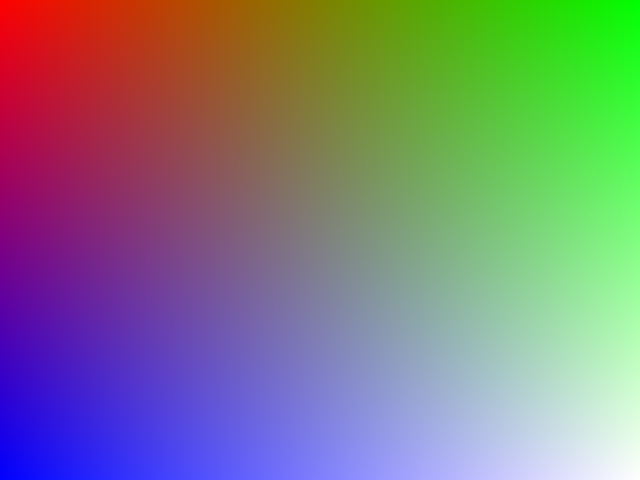
\includegraphics[width=0.7\textwidth]{gradient}
  \caption{A different map image that makes use of the used features.}
  \label{fig:newmap}
\end{figure}

In this case, the image was chosen by manual analysis of the
features. A more interesting case would be to generate the image based
on desired properties of the inverse correlation matrix. 

An ideal inverse correlation matrix would look like:

\begin{table}                                   
\centering                                      
\begin{tabular}{l|rrrrr}                    
    red   & 1.30  &       &       &       &      \\  
    green & -0.59 & 2.64  &       &       &      \\
    blue  & 0.02  & -1.81 & 2.37  &       &      \\ 
    x     & 0.14  & -0.02 & 0.01  & 1.02  &      \\ 
    y     & 0.13  & 0.24  & -0.32 & -0.01 & 1.06 \\ 
  \midrule
  $R^2$   & 0.23  & 0.62  & 0.58  & 0.02  & 0.06 \\
  \midrule
          & red   & green & blue  & x     & y
\end{tabular}                                   
\caption{Inverse correlation matrix}                        
\label{table:MyTableLabel}                      
\end{table} 

%$R^2$   & *  & *  & *  & 1.00  & 1.00 \\

One possible solution would be to set all correlations to a high
value.

\subsection{The backward approach}

\begin{figure}[h]
  \centering
  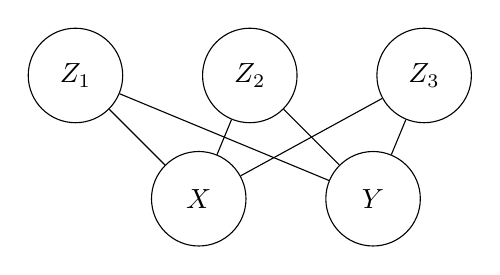
\begin{tikzpicture}[every node={}]
    \node[latent, minimum size=1.2cm] (z1) {$Z_1$} ; %
    \node[latent, right=of z1, minimum size=1.2cm] (z2) {$Z_2$} ; %
    \node[latent, right=of z2, minimum size=1.2cm] (z3) {$Z_3$} ; %
    \node[latent, below right=of z1, minimum size=1.2cm] (x) {$X$} ; %
    \node[latent, below right=of z2, minimum size=1.2cm] (y) {$Y$} ; %
    \edge[-] {z1} {x}; \edge[-] {z1} {y}; \edge[-] {z2} {x}; \edge[-]
    {z2} {y}; \edge[-] {z3} {x}; \edge[-] {z3} {y};
  \end{tikzpicture}
  \caption{The graphical model used for generating ideal images.}
\end{figure}

Knowing the criteria for computing $R^2$, we could construct optimal
images for the given approach. These images will be gradient
images. Since images consist of three channels, we could encode the
information in two channels, and use arbitrary information in the
third channel---and therefore even keep our initial image to a great
extent.

\subsection{Vine Copula}

In our final approach, we try to capture the dependence structure
without modifications of the original map image. In order to do, we
need a more powerful model. The use of \emph{copulas} allows to model
marginal distributions and dependence structure independently,
allowing for convenient and powerful representation of joint
probability distributions.
                                          
\section{Discussion}



\section{Conclusion}

In this report, the suitability of independence graphs for computer
vision-based localization was shown. While the straight-forward
application of linear regression was not able to capture the structure
in the generated dataset, a modification of the image underlying the
data set allowed to generate a simple and effective model, which lead
to low mean squared errors. Since the
modification of the underlying image might be undesired or not
possible, two more powerful approaches have been presented. The
Gaussian 

Future research will include the modeling of time dependence: in a
real-world scenario, successive images will be, leading a a Bayesian
network, as presented by Daphne.



\appendix

\section{Supplementary Material}

\section{Dataset with average red, green, and blue values}
\begin{center}
  \csvautotabular{../all_vals.csv}
\end{center}
\end{document}
